%----------------------------------------------------------------------------------------
%	PACKAGES AND OTHER DOCUMENT CONFIGURATIONS
%----------------------------------------------------------------------------------------
\documentclass[DIV=calc, paper=a4, fontsize=12pt, onecolumn]{scrartcl}	 % A4 paper and 12pt font size

\usepackage[english]{babel} % Engllish language /hyphenation
\usepackage[protrusion=true,expansion=true]{microtype} % Better typography
\usepackage{booktabs} % Horizontal rules in tables
\usepackage[svgnames]{xcolor} % Enabling colors by their 'svgnames'
\usepackage{fix-cm}	 % Custom font sizes - used for the initial letter in the document
\usepackage{graphicx} % Inserting figures and images
\usepackage{natbib}  % For using the APA bibliography style

\usepackage{sectsty} % Enables custom section titles
\allsectionsfont{\usefont{T1}{phv}{b}{n}} % Change the font of all section commands

\usepackage{fancyhdr} % Needed to define custom headers/footers
\pagestyle{fancy} % Enables the custom headers/footers
\usepackage{lastpage} % Used to determine the number of pages in the document (for "Page X of Total")
\usepackage{url} % Used to format urls correctly

% Headers - all currently empty
\lhead{}
\chead{}
\rhead{}

% Footers
\lfoot{}
\cfoot{}
\rfoot{\footnotesize Page \thepage\ of \pageref{LastPage}} % "Page 1 of 2"

\renewcommand{\headrulewidth}{0.0pt} % No header rule
\renewcommand{\footrulewidth}{0.4pt} % Thin footer rule

\usepackage{hyperref}
\hypersetup{
	colorlinks=true, %set true if you want colored links
	linktoc=all, %set to all if you want both sections and subsections linked
	linkcolor=blue, %choose some color if you want links to stand out
	citecolor=Maroon,
	urlcolor=SteelBlue, 
	}
	
\addto{\captionsenglish}{\renewcommand*\contentsname{Table of Contents}}

\usepackage{lettrine} % Package to accentuate the first letter of the text
\newcommand{\initial}[1]{ % Defines the command and style for the first letter
\lettrine[lines=3,lhang=0.3,nindent=0em,slope=0em]{
\color{DarkBlue}
{\textbf{\textit{#1}}}}{}}



%----------------------------------------------------------------------------------------
%	TITLE SECTION
%----------------------------------------------------------------------------------------

\usepackage{titling} % Allows custom title configuration

\newcommand{\HorRule}{\color{DarkGoldenrod} \rule{\linewidth}{1pt}} % Defines the gold horizontal rule around the title

\pretitle{\vspace{-150pt} \begin{flushleft} \HorRule \fontsize{40}{40} \usefont{OT1}{phv}{b}{n} \color{DarkRed} \selectfont} % Horizontal rule before the title

\title{Semantic Healthcare} % Your article title

\posttitle{\par\end{flushleft}\vskip 0.5em} % Whitespace under the title

\preauthor{\begin{flushleft}\large \lineskip 0.5em \usefont{OT1}{phv}{b}{sl} \color{DarkRed}} % Author font configuration

\newcommand{\org}{\footnotesize \usefont{OT1}{phv}{m}{sl} \color{Black}}

\DeclareRobustCommand{\authoring}{
\begin{tabular}{ccc}
  Sankhesh Jhaveri & Catherine Dumas & Joshua Cope\\
  \org Kitware,Inc. & \org SUNY Albany & \org SUNY Albany
\end{tabular}}

\author{\authoring} % Your name

\postauthor{\footnotesize \usefont{OT1}{phv}{m}{sl} \color{Black} % Configuration for the institution name
 % Your institution

\par\end{flushleft}\HorRule} % Horizontal rule after the title

\date{} % Add a date here if you would like one to appear underneath the title block

%\setcounter{secnumdepth}{0} % All sections start from depth 0

%----------------------------------------------------------------------------------------

\begin{document}

  \maketitle
  \renewcommand{\contentsname}{\hspace{120pt} Table of Contents}
  \tableofcontents
  \thispagestyle{fancy} % Enabling the custom headers/footers for the first page
  \vspace{20pt}
%----------------------------------------------------------------------------------------
%	SNOMED RT
%----------------------------------------------------------------------------------------
   \section[Systematized Nomenclature in Medicine  Reference Terminology (SNOMED RT\textsuperscript{\textregistered})]
   {SNOMED RT\textsuperscript{\textregistered}}
   \label{sec:snomedrt}
   
   \initial{S}\textit{ystematized Nomenclature in Medicine Reference Terminology\\ (SNOMED RT)}\
   represents the initial step towards unifying various clinical terms in healthcare. SNOMED RT was\
   designed to complement the broad coverage of medical concepts in SNOMED with a set of\
   enhanced features that significantly increased its value as a reference terminology for\
   representing clinical data~\citep{spackman_snomed_1997}. SNOMED RT was developed by\
   the College of American Pathologists (CAP).\\
   
  \noindent SNOMED RT is a concept-based terminology. A \emph{concept} is a unit\
  of thought that refers to a unique, clearly defined entity. An example is ``Fundus of stomach''.\
  \begin{table}[ht!]
    \centering
    \begin{tabular}{| l | l | l |}
      \hline
      Concept Code & Descriptions                      & Status \\ \hline \hline
      D3-89550        & Cerebrovascular accident & Preferred name\\
                              & CVA                                   & Synonym\\
                              & Stroke                               & Synonym\\                   
      \hline
      \end{tabular}
    \caption{SNOMED RT - Concepts, Descriptions and Synonyms}\citep[Table.~1]{a_y_wang_mapping_2001}
    \label{tab:snomedrt_example}
  \end{table}
  A \emph{term} is a particular lexical string or expression that represents a concept.\
  Terms are used in clinical information systems or other healthcare applications.\
  In SNOMED RT, we use \emph{description} to refer to terms that are linked\
  to concepts in core tables. This imparts a specific, nonambiguous meaning to each\
  term. A single concept may have one or more associated descriptions. One description\
  in each concept is designated the \emph{preferred name}, and the others are called\
  \emph{synonyms}(See Table~\ref{tab:snomedrt_example}). Term and description have often been used\
  interchangeably in the past. However, the two are being distinguished because\
  a term can be associated with different concepts in the clinical information\
  systems depending on context, but a description is ideally non-ambiguous\
  and always associated with a concept.\\
  
  \noindent Some of the fundamental aspects of SNOMED RT~\citep{dolin_snomed_2001} are:
  \begin{itemize}
    \itemsep0ex
    \item Hierarchies in SNOMED RT represent strict supertype-subtype relationships.\
    Therefore, a child concept is necessarily always a kind of the parent concept.
    \item Concepts are defined by their placement in a (poly)hierarchy and by additional\
    properties called ``Relationship Types'' or ``Roles'', whose target values are also\
    SNOMED concepts. For example, Appendectomy (P1-57450) has an\
    ``ASSOCIATED-TOPOGRAPHY'' role, whose value is Appendix (T-59200).
    \item SNOMED RT contains textual definitions, which are especially valuable when\
    the underlying description logic is unable to define a procedure fully.
  \end{itemize}
  
%----------------------------------------------------------------------------------------
%	SNOMED CT
%----------------------------------------------------------------------------------------

  \section[Systematized Nomenclature in Medicine Clinical Terms\\ (SNOMED CT\textsuperscript{\textregistered})]
  {SNOMED CT\textsuperscript{\textregistered}}
  \label{sec:snomedct}

  \initial{S}\textit{ystematized Nomenclature in Medicine Clinical Terms (SNOMED CT)}\
   is a comprehensive, multilingual clinical terminology that provides clinical content and\
   expressivity for clinical documentation and reporting. It can be used to code, retrieve\
   and analyze clinical data.\
   SNOMED CT was formed by the merger, expansion and restructuring of\
   SNOMED RT\textsuperscript{\ref{sec:snomedrt}}\
   and the United Kingdom National Health Service (NHS)\
   Clinical Terms (also known as the Read Codes).\
   In a nutshell, SNOMED CT consists of concepts arranged in a hierarchy, connected\
   by relationships. The International Health Terminology Standards Development Organization\
   (IHTSDO) owns and administers the rights to SNOMED CT.\\

  According to \citep{snomed_-_user_guide_snomed_2011}, there are three basic\
  components of SNOMED CT:
  \begin{itemize}
    \itemsep0ex
	  \item{Concepts}
	  \item{Descriptions}
	  \item{Relationships}
  \end{itemize}

  \subsection{Concepts}
  Concepts are clinical ideas, ranging from \emph{abscess} to \emph{zygote},\
  identified by a unique numeric identifier (\textit{ConceptId}) that never changes\
  and represented by a unique human readable \textit{Fully Specified Name (FSN)}.\
  The concepts are formally defined in terms of their Relationships with other concepts.\
  These logical definitions give explicit meaning which a computer can process and query\
  on. Every concept also has a set of terms that name the concept in a human-readable\
  way. There are well over 300,000 active concepts in the terminology with differing levels\
  of granularity linked to one another by \textbar ~is a \textbar ~relationships as depicted\
  in Figure~\ref{fig:snomedct_concepts_granularity}.\\
  \begin{figure}[!ht]
    \centering
    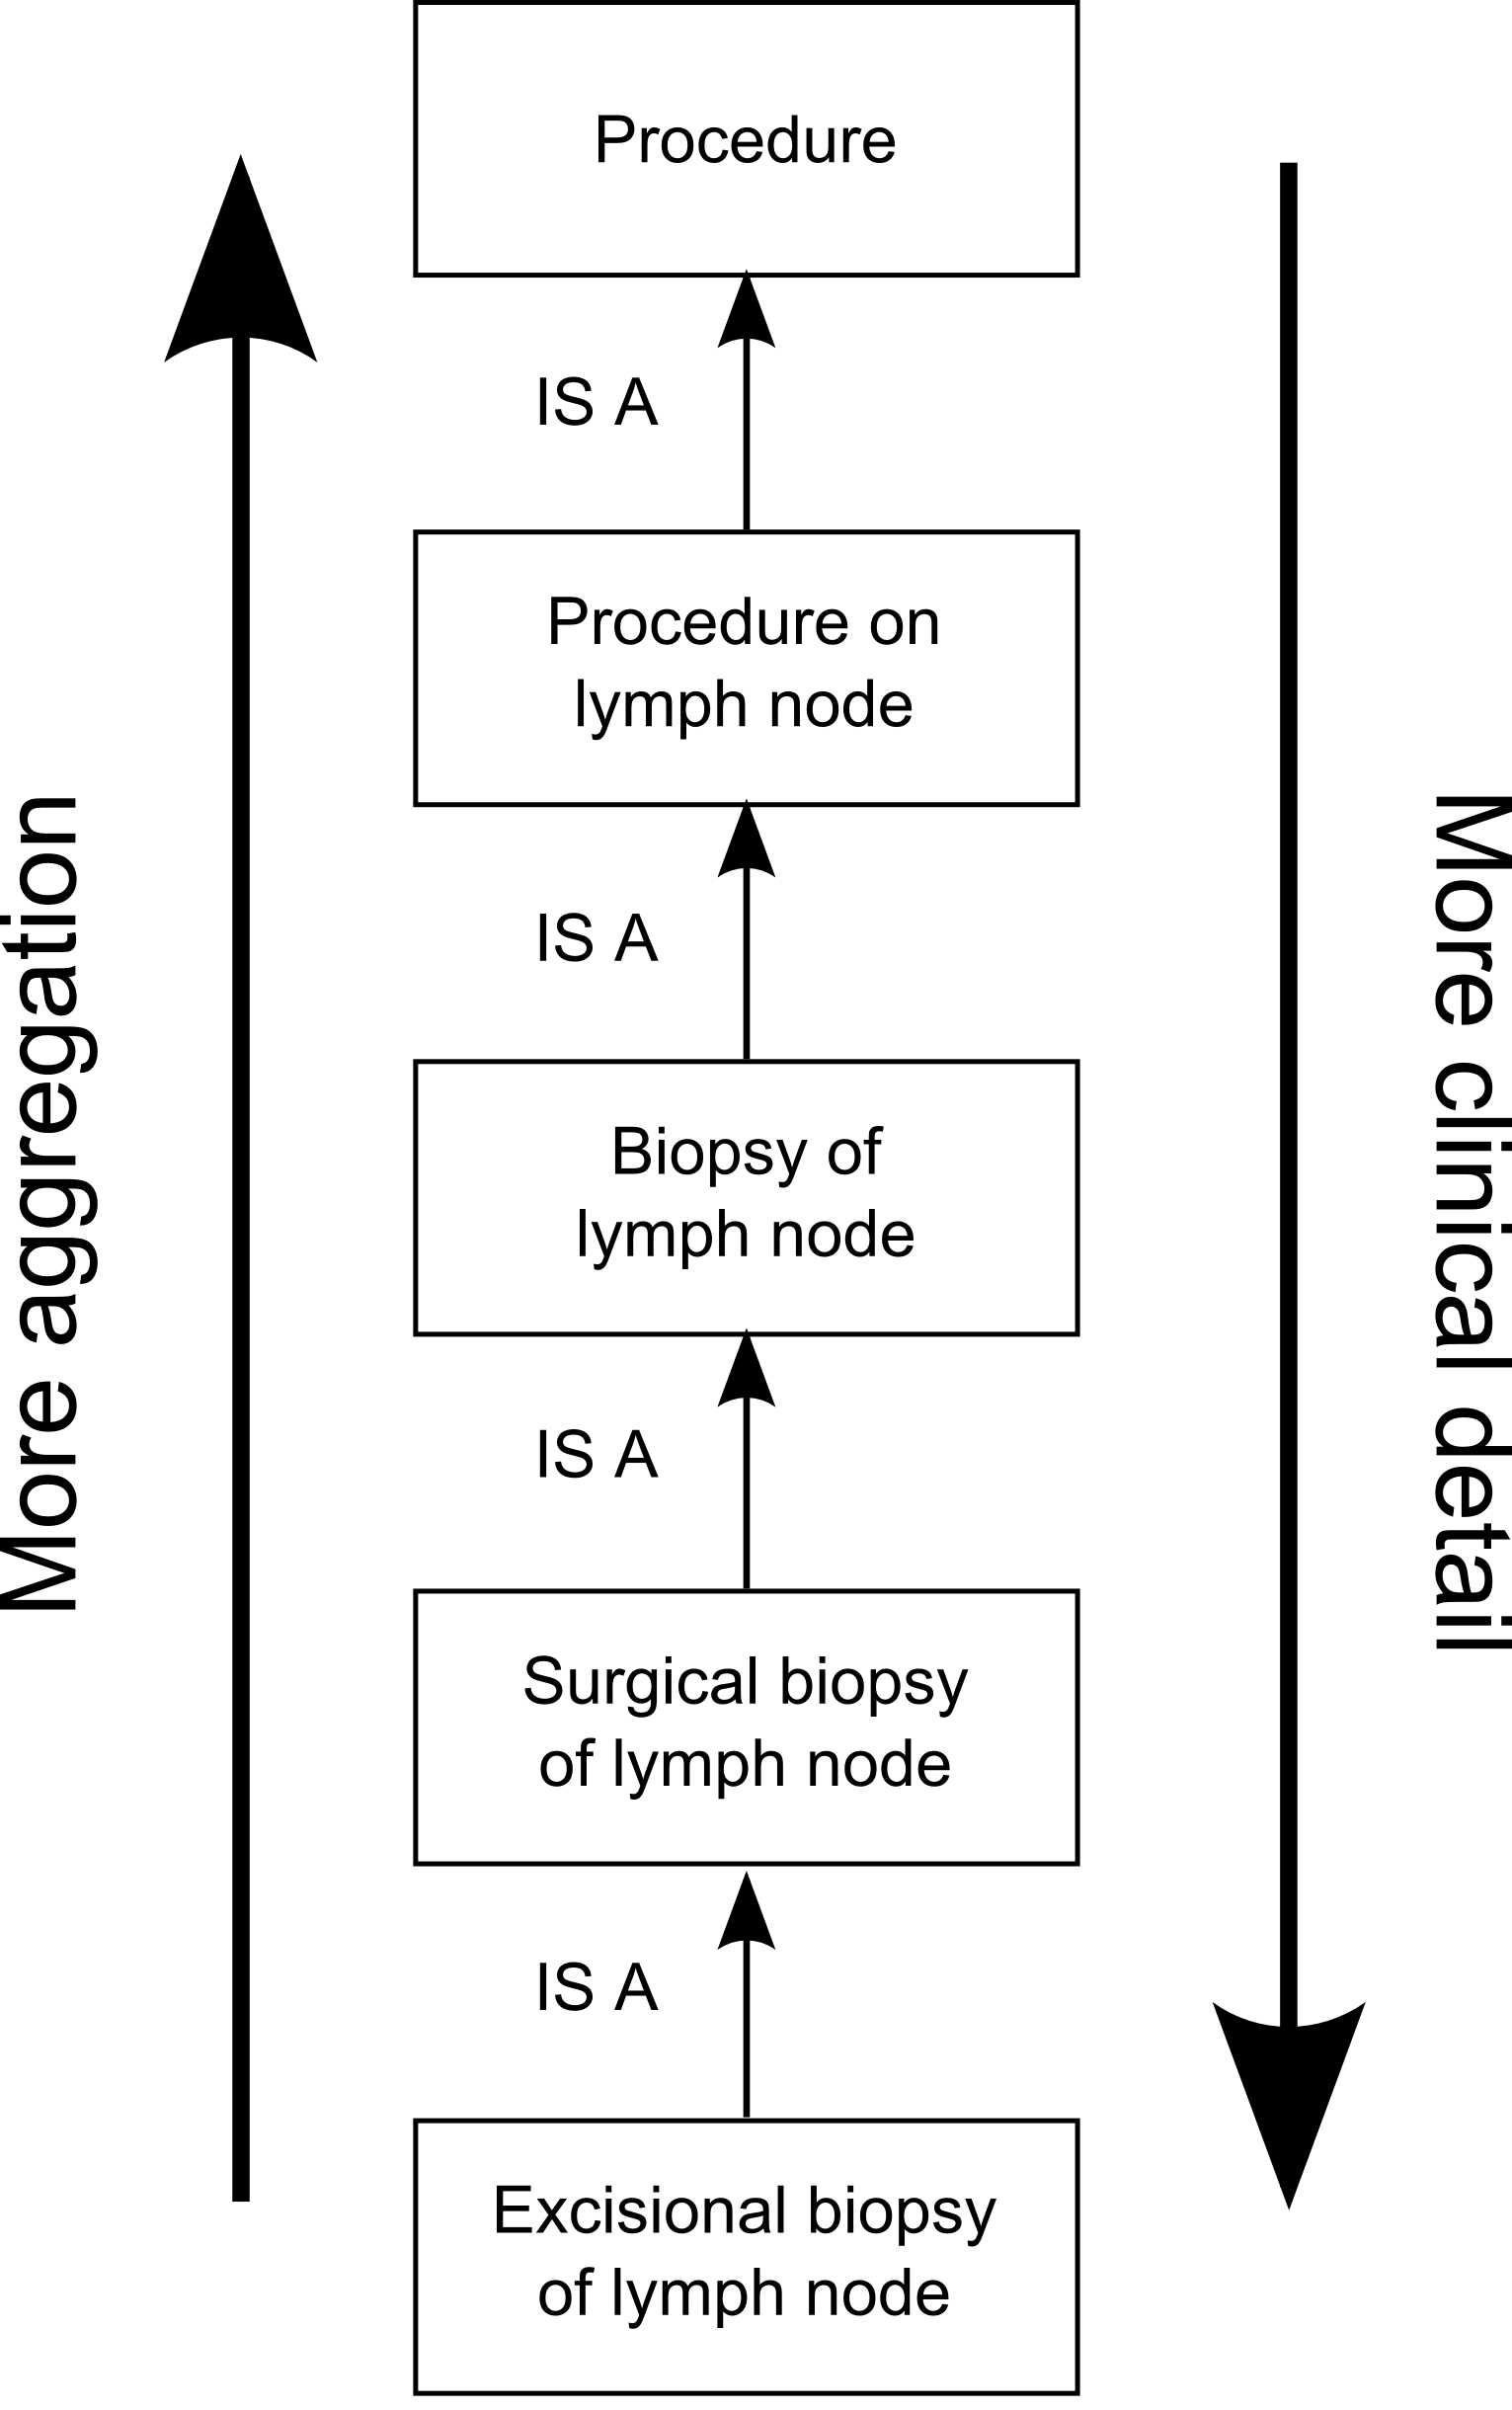
\includegraphics[scale=1]{granularity.png}
    \caption{SNOMED CT - Multiple levels of granularity}\citep[Fig.~1]{snomed_-_user_guide_snomed_2011}
    \label{fig:snomedct_concepts_granularity}
  \end{figure}

  \noindent Concept identifiers in SNOMED CT are meaningless to avoid changes to\
  reflect revised understanding of the nature of a disorder. Meaningless identifiers\
  also enable multiple aspects of meaning to be represented in the same way.\\
  
  \subsection{Descriptions}
  Concept Descriptions are the terms or names assigned to a SNOMED CT concept.\
  A unique DescriptionId  identifies a Description. Multiple Descriptions might be\
  associated with a concept identified by a ConceptId. There are nearly a million\
  English Descriptions in the International Release of SNOMED CT. Each translation\ 
  of SNOMED CT includes an additional set of descriptions, which link terms in another\
  language to the same SNOMED CT concepts.
  
  \noindent\textbf{\emph{Example:}}
  Some of the Descriptions associated with \emph{ConceptId} 22298006:
  \begin{itemize}
    \itemsep0ex
    \item{Fully Specified Name: | Myocardial infarction (disorder) | \emph{DescriptionId}\
    751689013}
    \item{Preferred term: Myocardial infarction \emph{DescriptionId} 37436014}
    \item{Synonym: Cardiac infarction \emph{DescriptionId} 37442013}
    \item{Synonym: Heart attack \emph{DescriptionId} 37443015}
    \item{Synonym: Infarction of heart \emph{DescriptionId} 37441018}
  \end{itemize}
  Each of the above Descriptions has a unique \emph{DescriptionId}, and all of these\
  Descriptions are associated with a single Concept (and the single \emph{ConceptId} 22298006).\\

  \subsection{Relationships}
  SNOMED CT Relationships link each concept to other concepts that have a related\
  meaning. These relationships provide formal definitions and other characteristics of\
  the concept. One type of link is the \textbar ~is a \textbar ~relationship which\
  relates a concept to the its more general concepts. For example (Figure~\ref{fig:snomedct_relationships}), the concept\
  ``viral pneumonia'' has an \textbar ~is a \textbar ~relationship to the more\
  general concept ``pneumonia''. These \textbar ~is a \textbar ~relationships\
  define the hierarchy of SNOMED CT concepts. Other types of relationships\
  represent other aspects of the definition of a concept. For example, the concept\
  ``bacterial pneumonia'' has a \textbar ~causative agent \textbar ~relationship to\
  the concept ``bacteria'' and a \textbar ~finding site \textbar ~relationship to the\
  concept ``lung structure''. There are well over a million relationships in SNOMED CT.
  \begin{figure}[!ht]
    \centering
    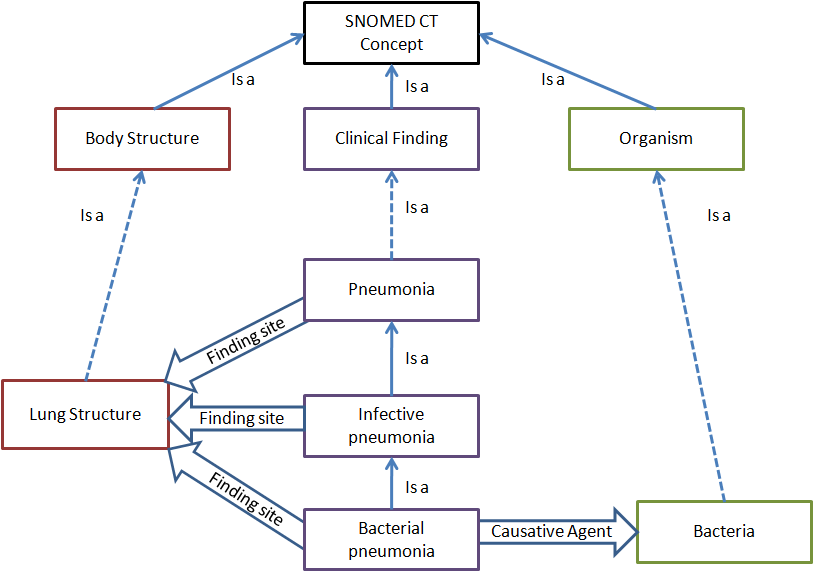
\includegraphics[scale=0.5]{defining_relationship_example1.png}
    \caption{SNOMED CT - Illustration of Defining Relationships}\citep[Fig.~7]{snomed_-_user_guide_snomed_2011}
    \label{fig:snomedct_relationships}
  \end{figure}

\subsection{Implementation}
  SNOMED CT is distributed as a set of tab-delimited text files that can be\
  imported into a relational database. The three tables - the Concepts table,\
  the Descriptions table and the Relationships table are commonly referred to\
  as \emph{Core Components}~\citep{snomed_implementation_guide_snomed_2011}.\
  Supplementary tables called \emph{Reference Sets} specify the common extensible\
  pattern that is used to add additional information related to the core components.

  \subsection{Summary}
  SNOMED CT is a used widely to achieve semantic uniformity\
  and consistency of health terms as well as to achieve interoperability between\
  HL7\textsuperscript{\ref{sec:fhir}}\
  (Health Level 7) based health frameworks and other healthcare entities as shown\
  by the works in \citep{ryan_towards_2006,arguello_executing_2009,khan_achieving_2012}.\
  Not only does it provide unique semantic identifiers to clinical concepts, SNOMED CT\
  also describes and links different concepts in an ontogolical fashion.\
  While SNOMED CT has emerged internationally as a leading terminology, the work of\
  \citep{he_clinical_2012, khare_exploiting_2012} delineates that the existing SNOMED CT\
  lexicon suffers from a surprisingly huge paucity of synonyms.\
  Efforts are underway to reduce SNOMED CT's structural complexity\
  and provide a metathesaurus of clinical concepts with mappings to different terminologies,\
  thereby improving semantic integrity in practical healthcare scenarios.\
  \citep{lindberg_unified_1993,wei_using_2012}
%----------------------------------------------------------------------------------------
%	CMT
%----------------------------------------------------------------------------------------
  \section[Convergent Medical Terminology (CMT)]{CMT}
  \label{sec:cmt}

  \initial{C}onvergent Medical Terminology (CMT) is a set of clinician and patient friendly\
  terminology, linked to US and international interoperability standards, and\
  related vocabulary development tools and utilities. Developed by Kaiser\-
  Permananente over many years for use within its health-IT systems, CMT now\
  includes more than 75,000 concepts. CMT is a core component Kaiser Permanente's\
  comprehensive electronic health record \emph{KP HealthConnect\textsuperscript\textregistered}.\\

  \begin{figure}[ht!]
    \label{fig:cmt}
    \centering
    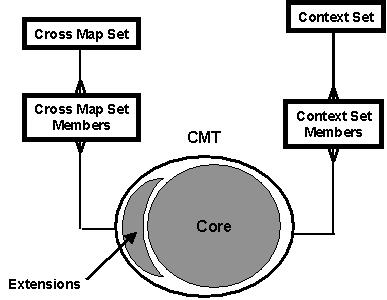
\includegraphics[scale=0.75]{CMT.jpg}
    \caption{High-level graphical description\
    of CMT}\citep[Fig.~1]{dolin_kaiser_2004}
  \end{figure}  

  \noindent In September 2010 Kaiser Permanente, the International Health\
  Terminology Standards Development Organisation (IHTSDO) and the US\
  Department of Health and Human Services jointly announced Kaiser Permanente's\
  donation of their CMT content and related tooling to the IHTSDO. The donation\
  consists of terminology content already developed, a set of tools to\
  help create and manage terminology and processes to control the quality of\
  terminology that is developed. CMT also includes mappings to classifications\
  and standard vocabularies including SNOMED CT\textsuperscript{\ref{sec:snomedct}}.\\
  
  \noindent A high-level graphical depiction of CMT\
  is shown in Figure~\ref{fig:cmt}. CMT is built upon\
  industry standard terminologies. SNOMED CT\textsuperscript{\ref{sec:snomedct}},\
  laboratory LOINC\textsuperscript{\ref{sec:loinc}} and First DataBank\textsuperscript{\ref{sec:fdb}} drug\
  terminology form the core of CMT. Core terminologies are integrated into a\
  single poly-hierarchically structured knowledge base. A classifier organizes\
  the CMT concepts into a poly-hierarchy, based on their definitions.\
  The act of classifying helps identify synonymous concepts, and maintains quality\
  and consistency across the some 400,000 concepts.\\
  
  \noindent Applications can directly access CMT via a provided interface and/or\
  CMT can provide applications with cross map sets and context sets, both of which\
  are patterned after the SNOMED CT\textsuperscript{\ref{sec:snomedct}} model.\
  Cross map sets are used to store mappings between CMT concepts and other coding schemes.\
  Context sets are CMT subsets used within a particular context. Contexts\
  can include a particular drop-down list or vocabulary table in an application,\
  a field in an HL7\textsuperscript{\ref{sec:fhir}} message, or any other CMT\
  subset needed within the organization.\\
  
  \noindent CMT is currently distributed within the UMLS Metathesauras\
  (\url{http://www.nlm.nih.gov/research/umls/knowledge_sources/metathesaurus/index.html}).
  
  
%----------------------------------------------------------------------------------------
%	RDF
%----------------------------------------------------------------------------------------


 \section[Resource Description Framework (RDF)]{RDF}
  \label{sec:rdf}

\initial{R}\textit{esource Description Framework (RDF)}\
is a World Wide Web Consortium (W3C) standardized data model for representing\
semantic Web resources. It uses graphs to represent information using a triple-based\
 notation comprising a subject, predicate and an object. All these entities can be uniquely identified by Internationalized Resource Identifiers (IRIs).\
  \citep{pathak_applying_2012}

\subsection{How we can use it}

We can use it by evoking already existing tools such as D2R Map\
  (\url{http://wifo5-03.informatik.uni-mannheim.de/bizer/d2rmap/D2Rmap.htm}),
 which is an open source tool thats transfers relational data into RDF\
 format which will then allow us to easily gain better insight between data.\

\subsection{Why this model would be useful for our application}

"RDF offers a practical evolutionary pathway to semantic interoperability. It enables information\
 to be readily linked and exchanged with full semantic fidelity while leveraging existing IT infrastructure investments.\
 Being schema-flexible, RDF allows multiple evolving data models and vocabularies to peacefully co-exist in the same instance\
data, without loss of semantic fidelity. This enables standardized data models and vocabularies to be used whenever possible\
, while permitting legacy or specialized models and vocabularies to be semantically linked and used when necessary. It also\
 enables a limitless variety of related information to be semantically linked to patient data, such as genomic, geographic and drug\
 interaction data, enabling more effective treatment, and greater knowledge discovery. Other reasons for adopting RDF as a universal\
 healthcare exchange language include:

\begin{description}
\item[(a)]  Its ability to make information self-describing with precise semantics
\item[(b)] its support for automated inference
\item[(c)]  its foundation in open standard"
\end{description}

 (\url{http://www.osehra.org/blog/rdf-universal-healthcare-language-0})\\

By using a standard language for data interchange, new research discoveries could be made\
more efficiently and effectively.\

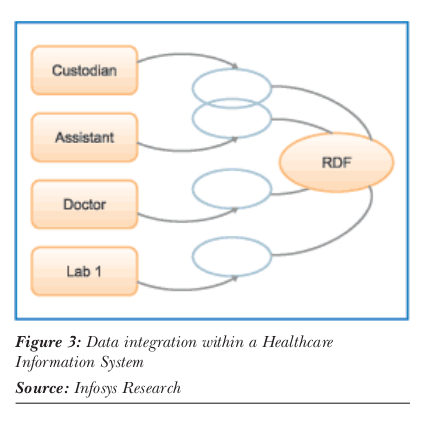
\includegraphics[scale=0.65]{rdfh.png}
 \citep{parachuri2008role}\\

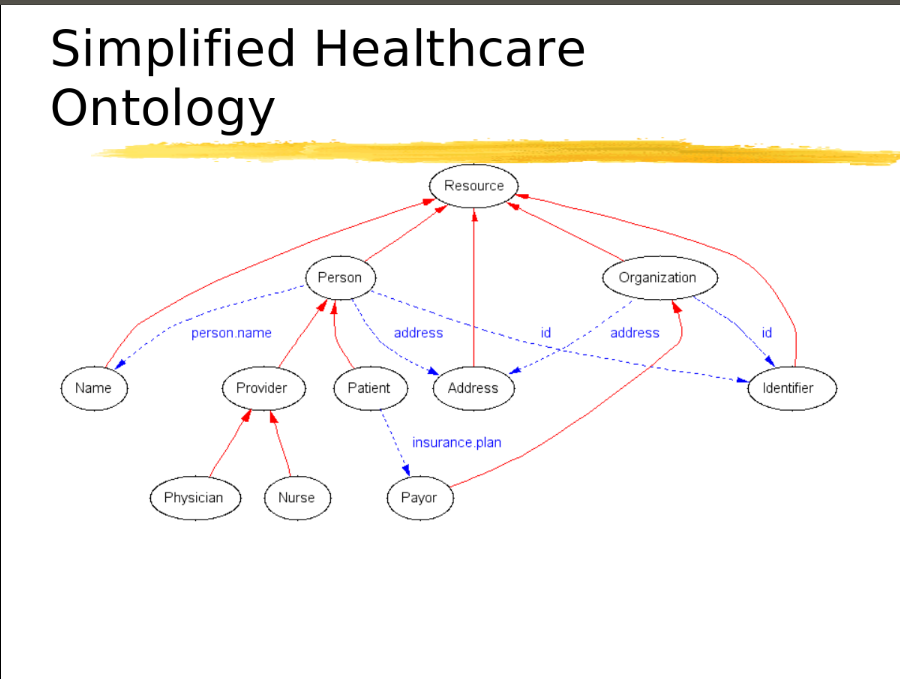
\includegraphics[scale=0.4]{rdf1.png}\\
 (\url{www.jonathanborden-md.com/HealthcareSemWeb.ppt‎})\\

\subsection{Comparison with other data models}

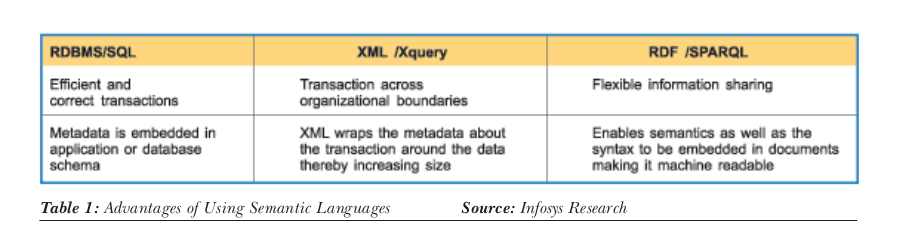
\includegraphics[scale=0.5]{sqlrdf.png}
 \citep{parachuri2008role}\\

XML:\\

XML is a comparable data model to RDF and in fact one way you can express RDF data is in a certain XML format.\
"What sets RDF apart from XML is that RDF is designed to represent knowledge in a distributed world.\
That RDF is designed for knowledge, and not data, means RDF is particularly concerned with meaning."\\

“In some ways, RDF can be compared to XML. XML also is designed to be simple and applicable to any type of data.\
XML is also more than a file format. It is a foundation for dealing with hierarchical, self-contained documents,\
 whether they be stored on disk in the usual brackets-and-slashes format, or held in memory and accessed through a DOM API."\\

 (\url{http://www.rdfabout.com/intro/})\\

SQL: \\

Relational Database’s such as SQL is also a comparable data model to RDF, and you can actually store your RDF data inside of a relational database.\
"Individual statements in RDF are expressed as subject, predicate, object triples. Sets of these with a common predicate\
 can be mapped to binary relations in the relational model, in the the common parlance, 2-column tables.”\\

"But a difference between the two is that in Relational DB's, for a certain set of values\
a relation is either considered either true (there is a corresponding row in the table) or false (there isn't).\
 In the RDF model in the general case, if a set of values isn't in the "row" (i.e. you don't have a particular statement), then it's not false, just unknown.”\\

 (\url{http://www.rdfabout.com/comparisons.xpd})\\

%----------------------------------------------------------------------------------------
%	Bio2RDF
%----------------------------------------------------------------------------------------
  \section{Bio2RDF}
  \label{sec:bio2rdf}
  
  \initial{B}\textit{io2RDF} is an open source project that uses semantic web\
  technologies to build and provide the largest network of Linked Data for the\
  Life Sciences. It defines a set of simple conventions to create\
  RDF\textsuperscript{\ref{sec:rdf}}\
  compatible Linked Data from a diverse set of heterogeneously formatted\
  sources obtained from multiple data providers. Bio2RDF is the culmination\
  of efforts towards addressing the pressing need for a global multisite\
  search engine. It is defined as a system that is able to query and connect\
  different databases available on the Internet~\citep{belleau_bio2rdf:_2008}.\\
    
  \begin{figure}[ht!]
    \centering
    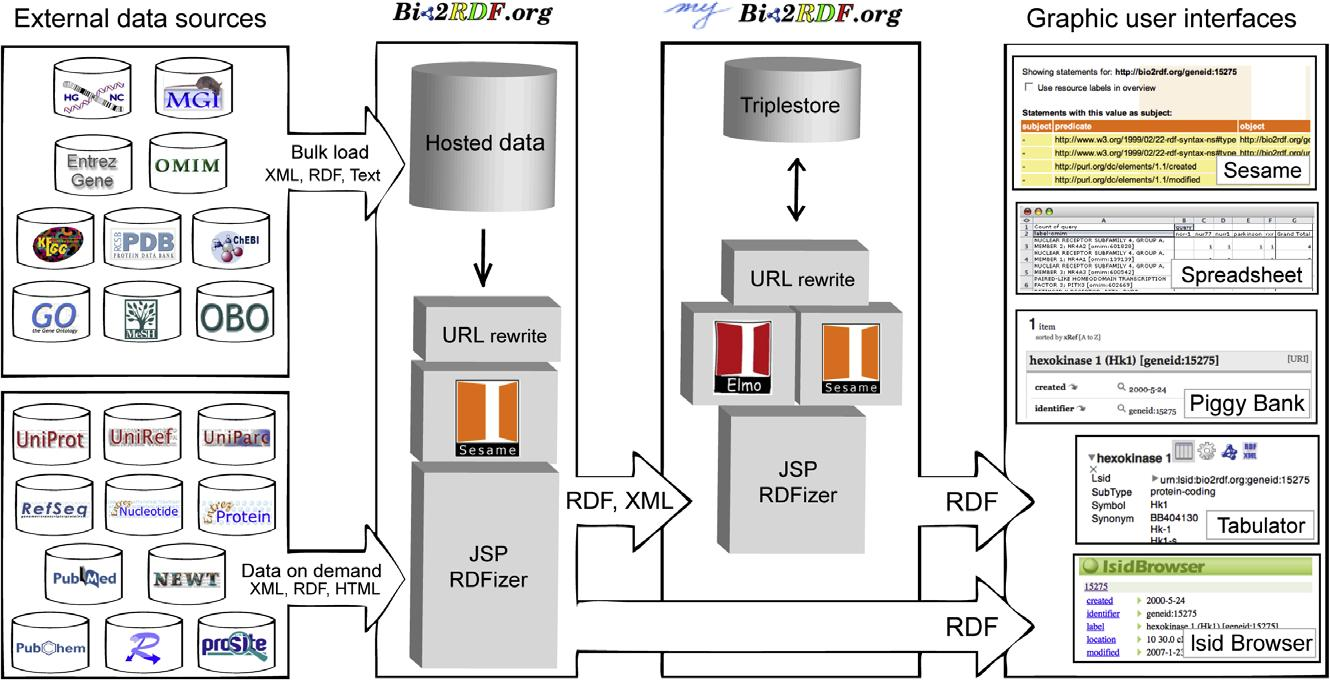
\includegraphics[scale=0.30]{bio2rdf_architecture.jpg}
    \caption{Bio2RDF knowledge system framework\
    architecture~\citep[Fig.~1]{belleau_bio2rdf:_2008}}
    \label{fig:bio2rdf_architecture}
  \end{figure}  

  \noindent Bio2RDF uses RDF documents and a\
  list of rules\
  (\emph{Banff Manifesto\footnote{\url{http://sourceforge.net/apps/mediawiki/bio2rdf/index.php?title=Banff_Manifesto}}})\
  to create URIs that will produce linked data:
  \begin{itemize}
    \itemindent3em
    \itemsep0ex
    \item [\textbf{Rule 1:}] URI's are normalized and dereferencable
    \item [\textbf{Rule 2:}] Autoritative public namespaces are used 
    \item [\textbf{Rule 3:}] Mandatory predicates are used
    \item [\textbf{Rule 4:}] Blank nodes are forbidden
    \item [\textbf{Rule 5:}] RDFizer programs are open source
    \item [\textbf{Rule 6:}] Deferenceable ontologies
  \end{itemize}
  Figure~\ref{fig:bio2rdf_architecture} shows a schematic description\
  of the Bio2RDF architecture. All external data sources, in different formats\
  (XML, Text, ASN.1, KGML and RDF), are listed on the left part. Data is then\
  made accessible either on the Bio2RDF.org server or on demand from the\
  original source. The myBio2RDF application contains an rdfizer program\
  and a servlet that answers Bio2RDF HTTP requests by formulating\
  SPARQL\textsuperscript{\ref{sec:sparql}} endpoints~\citep{callahan_bio2rdf_2013}.\\
  
  \subsection{Naming Convention}
  Bio2RDF entities are named as follows:
  \begin{quote}
    \url{http://bio2rdf.org/namespace:identifier}
  \end{quote}
  \noindent where, \emph{namespace} is the preferred short name of a\
  biological dataset and \emph{identifier} is the unique string used\
  by the source provider to identify the given record. For example,\
  HUGO Gene Nomenclature Committee identifies the human prostaglandin\
  E synthase gene (PIG12) with the accession number `9599'. This\
  dataset's namespace is ``hgnc'' in Bio2RDF's dataset\
  registry\footnote{\url{https://docs.google.com/spreadsheet/ccc?key=0AnGgKfZdJasrdElfQzRWWWhKUFR0UnRpeG14NGZRS2c}}\
  and the corresponding Bio2RDF IRI is:~\url{http://bio2rdf.org/hgnc:9599}\
  There are over 1800 such namespaces.
  
  \subsection{Bio2RDF Dataset Provenance Model}
  Provenance data for each Bio2RDF dataset is stored in a separate named\
  graph in each corresponding SPARQL endpoint. The provenance graph URI\
  follows the pattern:
  \begin{quote}
    \url{http://bio2rdf.org/bio2rdf-[dataset]-provenance}    
  \end{quote}
  \noindent where, `dataset' is the preferred short name (or prefix) for a given source\
  dataset as extracted from the Life Science Registry\footnote{Hosted by Bio2RDF\
  at \url{https://docs.google.com/spreadsheet/ccc?key=0AmzqhEUDpIPvdFR0UFhDUTZJdnNYdnJwdHdvNVlJR1E}}.\
  
  \begin{figure}[ht!]
    \centering
    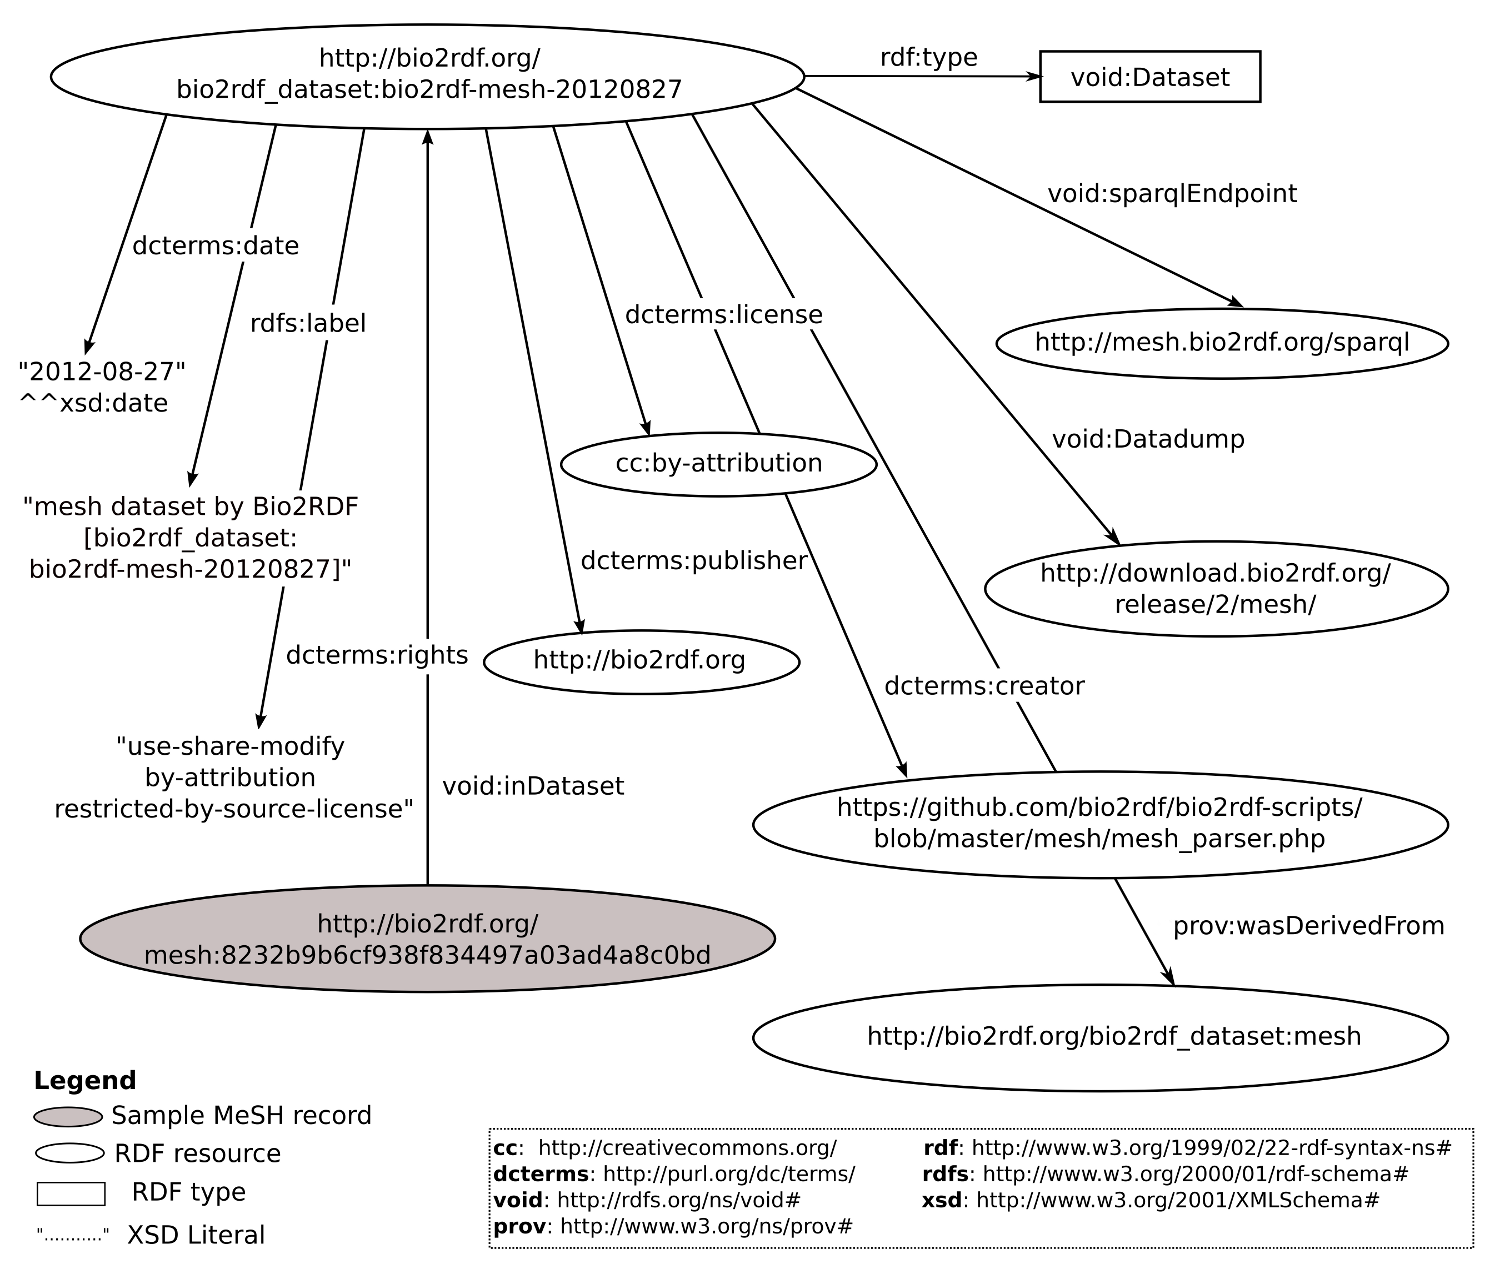
\includegraphics[scale=2.80,trim=1 1 1 1,clip]{bio2rdf_provenance.png}
    \caption{Bio2RDF Provenance Graph for the NLM Medical Subject Headings (MeSH)\
    architecture~\citep{bio2rdf_wiki_bio2rdf_2013}}
    \label{fig:bio2rdf_provenance}
  \end{figure}  
  
  \noindent For example, the ``NLM Medical Subject Headings (MeSH)'' dataset\
  provenance graph makes use of \url{http://bio2rdf.org/bio2rdf-mesh-provenance}\
  as its graph URI. Bio2RDF's provenance model uses the W3C Vocabulary of\
  Interlinked Datasets (VoID), the Provenance vocabulary (PROV) and\
  Dublin Core vocabulary.\
  Each dataset provenance object has a unique IRI and label based on the\
  dataset name and creation date. For example,\
  \url{http://bio2rdf.org/bio2rdf_dataset:bio2rdf-mesh-20120827}.\
  An example provenance graph for the MeSH dataset can be in figure~\ref{fig:bio2rdf_provenance}.\
  Note that each subject IRI in the dataset is linked the date-unique dataset\
  IRI that is part of the provenance record using the VoID `inDataset' predicate.\
  Other important features of the provenance record include the use of the Dublin\
  Core `creator' term to link a dataset to the script on Github that was used to\
  generate it, the VoID predicate `sparqlEndpoint' to point to the dataset SPARQL\
  endpoint, and VoID predicate `dataDump' to point to the data download URL.\\
  
  \noindent Although Bio2RDF facilitates integration of and programmatic access\
  to otherwise heterogeneous datasets (in both, content and format), a complete\
  syntactic and semantic normalization across numerous datasets has yet to be\
  fully realized. Works of~\citep{ansell_model_2011, callahan_ontology-based_2013}\
  demonstrate better and improved models of resolving queries to the Bio2RDF datasets.\\

%----------------------------------------------------------------------------------------
%	HDD
%----------------------------------------------------------------------------------------

\section[3M\textsuperscript{\texttrademark} Healthcare Data Dictionary (HDD)]
{3M HDD\textsuperscript{\texttrademark}}
  \label{sec:hdd}
  
  \initial{H}\textit{ealthcare Data Dictionary (HDD )}\
 is a controlled medical vocabulary server; makes it possible to map and manage medical terminologies, integrate content \& standardize healthcare data. Allows organizations to transmit \& receive accurate, actionable patient data across systems \& applications, regardless of where data originates% \citep{
  
  \subsection{How we can use it}\

\subsection{How is data stored}\


%----------------------------------------------------------------------------------------
%	ICD
%----------------------------------------------------------------------------------------

\section[International Classification of Diseases (ICD) ]{ICD}
  \label{sec:icd}

\initial{I}\textit{nternational Classification of Diseases (ICD)}\\

\subsection{How we can use it}\


\subsection{How is data stored}\

%----------------------------------------------------------------------------------------
%	LOINC
%----------------------------------------------------------------------------------------

\section[Logical Observation Identifier Names and Codes terminology (LOINC\textsuperscript{\textregistered})] 
{LOINC\textsuperscript{\textregistered}}
  \label{sec:loinc}
  
\initial{L}\textit{ogical Observation Identifier Names and Codes terminology (LOINC )}\\



\subsection{How we can use it}\

There is a free software program developed by The Regenstrief Institute called RELMA (the Regenstrief LOINC Mapping Assistant) which enables browsing and searching the database, review accessory content for terms and map local terms to LOINC \citep{kroth_using_2012} 

\subsection{How is data stored}\

%----------------------------------------------------------------------------------------
%	HL7/FHIR
%----------------------------------------------------------------------------------------

\section[Fast Healthcare Interoperability Resources (HL7 FHIR\textsuperscript{\texttrademark})]
{HL7 FHIR \textsuperscript{\texttrademark}}
  \label{sec:fhir}

\initial{F}\textit{ast Healthcare Interoperability Resources (HL7/FHIR )}\
is a is a next generation standards framework created by HL7.\
"It defines a set of "resources" for health. These resources represent granular clinical\
concepts that can be exchanged in order to quickly and effectively solve problems in healthcare\
 and related process. The resources cover the basic elements of healthcare - patients, admissions,\
diagnostic reports, medications, and problem lists, with their typical participants, and also support\
a range of richer and more complex clinical models. The simple direct definitions of the resources are\
 based on thorough requirements gathering, formal analysis and extensive cross-mapping to other relevant standards."\\
  (\url{http://www.hl7.org/implement/standards/fhir/v0.01/print-introduction.htm})\\

"Resources are:\

\begin{itemize}
\item Atomic - they are the smallest defined unit of operation and a transaction scope of their own.
\item Connected - resources refer to other resources to allow for clean modular reuse of information.
\item Independent - the content of a resource can be processed without having to retrieve referenced resources.
\item Simple - each resource definition is easy to understand, and to implement without needing specialized tooling or infrastructure (though that can be used if desired).
\item RESTful - resources are able to be used in a RESTful exchange context.
\item Flexible - resources can also be used in non-RESTful contexts, such as messaging or SOA architectures and can be moved in and out of RESTful paradigms as convenient.
\item Extensible - resources can be extended to allow for local requirements without impacting on interoperability.
\item Webcentric - where possible and appropriate, open internet standards are used for data representation.
\item Free for use - the FHIR specification itself is open - anyone can implement FHIR or derive related specifications without any IP restrictions.
\end{itemize}

In addition to the basic resources, FHIR defines a lightweight implementation framework that\
supports the use of these resources in RESTful environments, classic message exchanges, human-centric\
 clinical documents and enterprise SOA architectures. Each of these approaches provides its own benefits\ 
- FHIR provides the underpinning enablement that makes the choosing one of these painless and enables enterprises\
 to choose their own paradigm without forsaking interoperability with other approaches.\\

Though the resources are simple and easy to understand, they are backed by a thorough, global requirements gathering\
 and formal modeling process that ensures that the content of the resources is stable and reliable. The resource\
contents are mapped to solid underlying ontologies and models using computable languages (including RDF) so\
that the definitions and contents of the resources can be leveraged by computational analysis and conversion processes.\\

FHIR also provides an underlying conformance framework and tooling that allows different implementation contexts\ 
and enterprises to describe their context and use of resources in formal computable ways and to empower computed\
 interoperability that leverages both the conformance and definitional frameworks.\\

The combination of the resources and the 3 supporting layers (implementation frameworks,\
definitional thoroughness, and conformance tooling), along with the completely free license of FHIR\
 itself frees healthcare data so that it can easily flow to where it needs to be (across hospital production systems,\
 mobile clinical systems, cloud based data stores, national health repositories, research databases, etc.)\
without having to pass through format and semantic inter-conversion hurdles along the way.”\\
 (\url{http://hl7.org/implement/standards/fhir/overview.htm})


%----------------------------------------------------------------------------------------
%	NwHIN
%----------------------------------------------------------------------------------------

\section[Nationwide Health Information Network (NwHIN)]{NwHIN}
  \label{sec:nwhin}

\initial{``N}\textit{ationwide Health Information Network (NwHIN )}\
is a set of standards, services, and policies that enable the secure exchange\
of health information over the Internet.''\\
(\url{http://www.healthit.gov/policy-researchers-implementers/nationwide-health-information-network-nwhin})\\

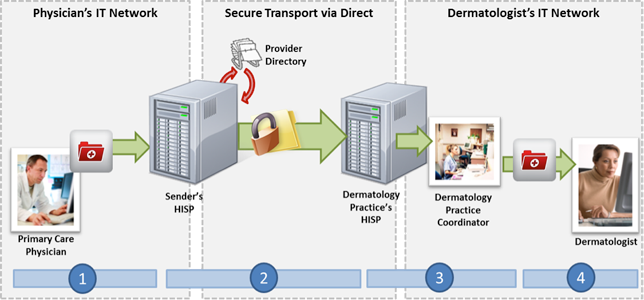
\includegraphics[scale=0.5]{nwhin.png}\\\
(\url{http://www.siframework.org/scenario_toc2.html})\

%----------------------------------------------------------------------------------------
%	SPARQL
%----------------------------------------------------------------------------------------

\section[SPARQL Protocol and RDF Query Language (SPARQL)]{SPARQL}
  \label{sec:sparql}

\initial{S}\textit{SPARQL Protocol and RDF Query Language (SPARQL)}\
		is a W3C recommend standard for querying RDF data.\
		It allows one to query remote RDF resources, in a manner similar to the querying of databases using SQL.\
		A SPARQL query is a set of graph patterns; any data triple matching these patterns is added to the query results.\
                   \citep{Jarrar_mashql:_2008}     
		
		\subsection{Alternatives}

		SquishQL - A simple RDF query language for beginners that allows for SQL syntax.\\
		(\url{http://www.techrepublic.com/article/squishql-the-simplest-rdf-query-language/})\

		\subsection{Examples}

                  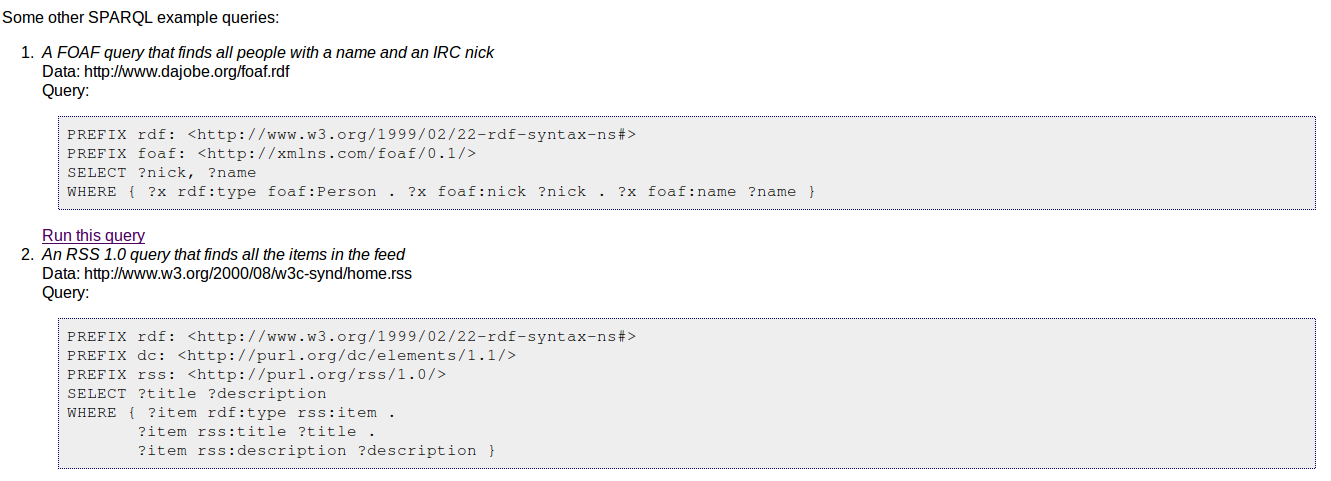
\includegraphics[scale=0.5]{sparql.png}\\
		 (\url{http://librdf.org/query/})

  		   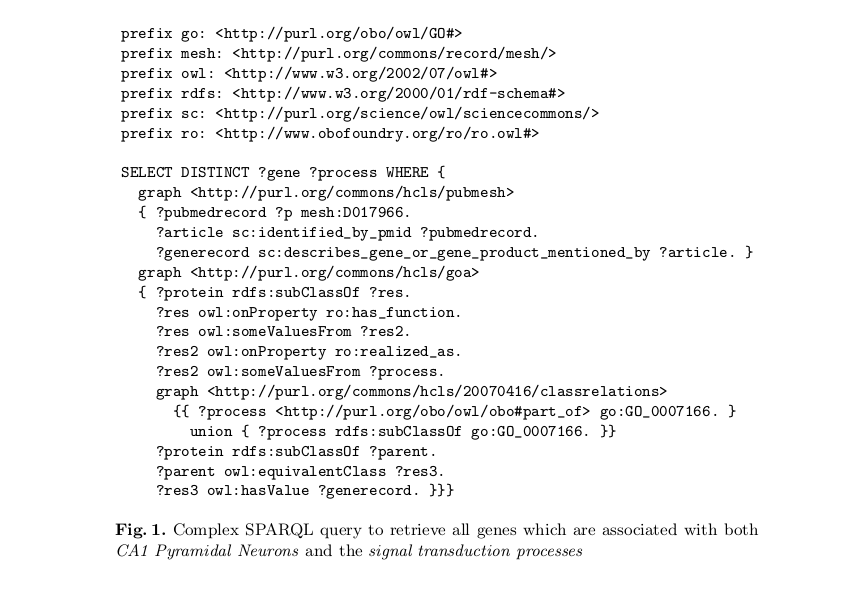
\includegraphics[scale=0.5]{sparql1.png}
 		  \citep{stenzhorn2008simplifying}\\

		  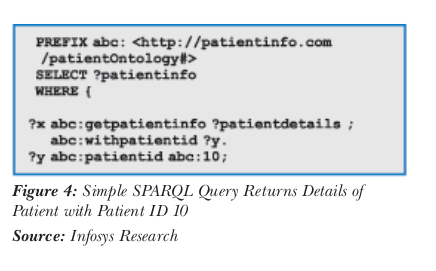
\includegraphics[scale=0.5]{sparqlh.png}
 		  \citep{parachuri2008role}
 		

		

%----------------------------------------------------------------------------------------
%	FMQL
%----------------------------------------------------------------------------------------

\section[FileMan Query Language (FMQL)]{FMQL}
  \label{sec:fmql}

\initial{F}\textit{ileMan Query Language (FMQL)}\
"is a Query Language that provides access to both FileMan data\
- a vital measurement of a patient - and the schema of that data - the type "Vital Measurement".\
The three things that it addresses are:
\begin{enumerate}
\item
Identity: every entity and entity type in FileMan gets a unique identifier - a URI.
\item
Data Formats: a consistent form of JSON, the web-friendly response format, for every type of data in the system\
 as well as HTML for human readers and RDF for web-data practitioners.
\item
Query Nuance: from the precise - SELECT - to the broader - DESCRIBE - or just COUNT, covers data hierarchies\
 and graphical layouts, paging and filtering."
\end{enumerate}
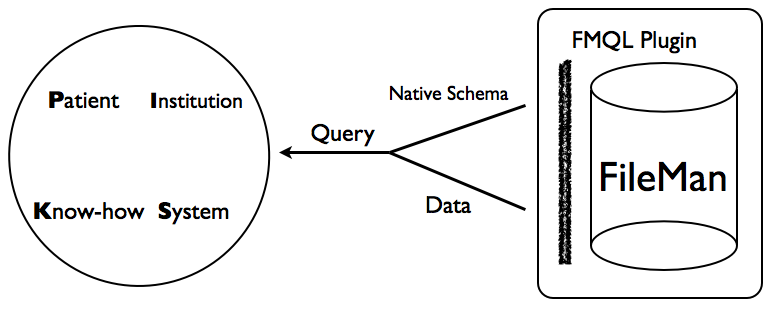
\includegraphics[scale=0.4]{fmqlFromFileMan.png}\\
(\url{http://vista.caregraf.info/fmql})\

%----------------------------------------------------------------------------------------
%	Miscellaneous Technologies
%----------------------------------------------------------------------------------------
\section{Miscellaneoous Technologies}
\label{sec:misc}

There have been multiple efforts undertaken to unify healthcare semantics.\
Some of the other technologies and/or lexicons that are being used currently\
are summarized here:

\subsection{First DataBank\textsuperscript{\texttrademark}}
\label{sec:fdb}
First Databank Inc.\footnote{\url{http://www.fdbhealth.com}},\
currently owned by Hearst Corporation, is a publisher\
of pharmaceutical industry market information and information\
technology. First Databank's proprietary knowledge base -\ 
\emph{MedKnowledge}~\citep{first_databank_fdb_2013}\
provides prices, descriptions, and collateral clinical information on drugs\
approved by the US Food and Drug Administration (FDA), plus commonly used\
over-the-counter drugs, herbal remedies, nutraceuticals and dietary supplements.\\

%----------------------------------------------------------------------------------------
%	REFERENCE LIST
%----------------------------------------------------------------------------------------

  \bibliographystyle{apa-good}
  \bibliography{SemanticHealthcare}{}

%----------------------------------------------------------------------------------------

\end{document}
